\documentclass[letterpaper, 10 pt, conference]{templates/ieeeconf}  % For letter paper

% \documentclass[a4paper, 10pt, conference]{templates/ieeeconf}      % For A4 paper

\IEEEoverridecommandlockouts                              % This command is only needed if
                                                          % you 2want to use the \thanks command

\overrideIEEEmargins                                      % Needed to meet printer requirements.

%% Add required packages %%
\usepackage{amsmath} 					% Assumes amsmath package installed
\usepackage{epsfig} 					% For postscript graphics files
\usepackage{cite} 						% For multiple citations
\usepackage{subfig} 					% For multiple figures
\usepackage{float} 						% To force position of floats
\usepackage{algorithm,algorithmic} 		% For algorithm table
\usepackage{hyperref} 					% To add url link in footnotes
\usepackage{array} 						% For tables
\usepackage{verbatim}  					% Needed for the "comment" environment to make LaTeX comments
\usepackage{caption}
\usepackage{multirow}
\usepackage[section]{placeins}
\usepackage{lipsum}
\usepackage{booktabs}
\usepackage{mathtools} 					% For cases eq
\usepackage{tikz} 						% For numbered circles

%% Add custom commands %%
\newcommand{\ra}[1]{\renewcommand{\arraystretch}{#1}}
\newcommand\T{\rule{0pt}{2.0ex}}        % Top strut
\newcommand\B{\rule[-0.4ex]{0pt}{0pt}}  % Bottom strut
\newcommand*\circled[1]{\tikz[baseline=(char.base)]{
		\node[shape=circle,draw,inner sep=1pt] (char) {#1};}} % For numbered circles
\DeclarePairedDelimiter{\nint}\lfloor\rceil % For integer rounding

% Algorithmic modifications
\makeatletter
\newcommand{\ALOOP}[1]{\ALC@it\algorithmicloop\ #1%
	\begin{ALC@loop}}
	\newcommand{\ENDALOOP}{\end{ALC@loop}\ALC@it\algorithmicendloop}
\renewcommand{\algorithmicrequire}{\textbf{Input:}}
\renewcommand{\algorithmicensure}{\textbf{Output:}}
\newcommand{\algorithmicbreak}{\textbf{break}}
\newcommand{\BREAK}{\STATE \algorithmicbreak}
\makeatother
\setlength{\tabcolsep}{4pt}
\hypersetup{urlcolor=black, colorlinks=false}  % Colours hyperlinks in blue, but this can be distracting if there are many links.

%% Define figure path %%
\graphicspath{{figures/}}

%%% Main text %%%%%%%%%%%%%%%%%%%%%%%%%%%%%%%%%%%%%%%%%%%%%%%%%%%%%%%%%%%%%%%%%%%%%%%%%%%%%%%%%

%%% Header %%%%%%%%%%%%%%%%%%%%%%%%%%%%%%%%%%%%%%%%%%%%%%%%%%%%%%%%%%%%%%%%%%%%%%%%%%%%%%%%%

\title{\LARGE \bf
IEEE Conference paper template
}

\author{
	Patiphon Narksri$^{1}$
\thanks{$^{1}$Graduate School of Informatics, Nagoya University, Furo-cho, Chikusa-ku, Nagoya, 464-8601, Japan}%
}

%%% Header %%%%%%%%%%%%%%%%%%%%%%%%%%%%%%%%%%%%%%%%%%%%%%%%%%%%%%%%%%%%%%%%%%%%%%%%%%%%%%%%%

%%% Contents %%%%%%%%%%%%%%%%%%%%%%%%%%%%%%%%%%%%%%%%%%%%%%%%%%%%%%%%%%%%%%%%%%%%%%%%%%%%%%%%%

\begin{document}
\maketitle
\thispagestyle{empty}
\pagestyle{empty}

% !TeX root = ../article.tex

\begin{abstract}

\lipsum[1]

\end{abstract}
% !TeX root = ../article.tex

\section{INTRODUCTION}

\lipsum[1-3]

\begin{figure}[!t]
    \centering
    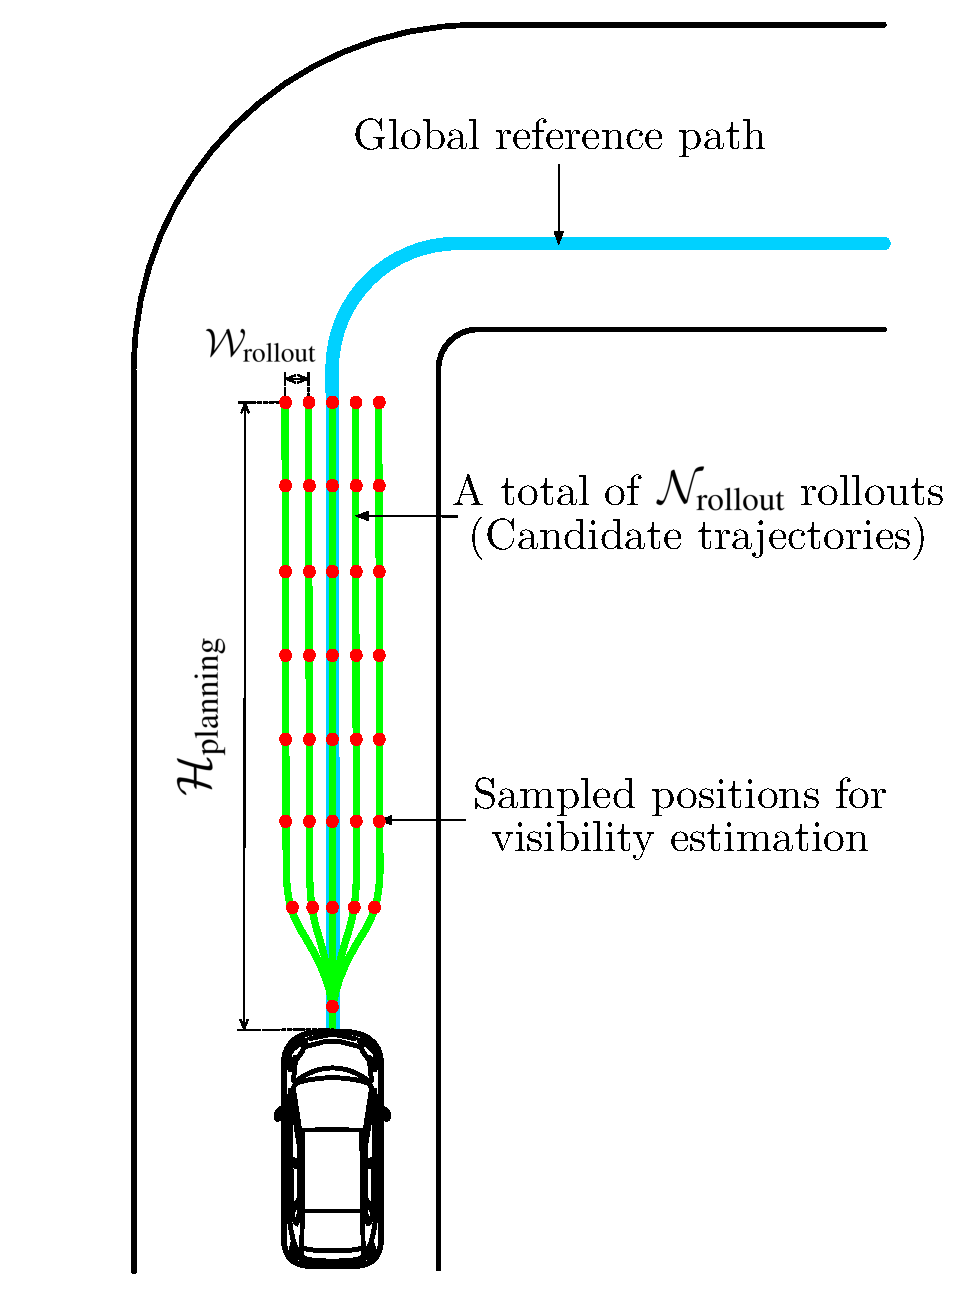
\includegraphics[width=0.75\linewidth]{rollout_generation}
    \caption
    {
        A sample figure from \cite{narksri_occlusion-aware_2022}.
    }
\end{figure}
% !TeX root = ../article.tex

\section{RELATED WORK}

\lipsum[4-5]
% !TeX root = ../article.tex

\section{PROPOSED METHOD}

\lipsum[7-10]
% !TeX root = ../article.tex

\section{EXPERIMENTS}

\lipsum[10-13]
\section{CONCLUSION}

\lipsum[14]

\addtolength{\textheight}{-0.9cm}   % This command serves to balance the column lengths
% on the last page of the document manually. It shortens
% the textheight of the last page by a suitable amount.
% This command does not take effect until the next page
% so it should come on the page before the last. Make
% sure that you do not shorten the textheight too much.

%%% Contents %%%%%%%%%%%%%%%%%%%%%%%%%%%%%%%%%%%%%%%%%%%%%%%%%%%%%%%%%%%%%%%%%%%%%%%%%%%%%%%%%

\section*{Acknowledgment}
This work was supported by xxxx.

%%% Main text %%%%%%%%%%%%%%%%%%%%%%%%%%%%%%%%%%%%%%%%%%%%%%%%%%%%%%%%%%%%%%%%%%%%%%%%%%%%%%%%%

\def\url#1{} % To disable URL in the references
\bibliographystyle{templates/IEEEtran}
\bibliography{bib/article}

\end{document}
\grid